\chapter{User Matrix in Recommendation Systems}\label{ch:user-matrix}

\index{Matrix Factorisation|(}

Matrix Factorization algorithms are generally classified as a collaborative filtering algorithms that are generally used in User Recommendation Systems. This type of algorithm generally works by performing a decomposition of the interaction matrix between the user and the item into the product of two lower dimensionality rectangular matrices \citep{Koren2006},

Modern day consumers are spoilt for choice as content providers offer a massive selection of products and options which can cater to a wide array of interests and tastes. Matching the appropriate product to the right customer is essential to improve client satisfaction, for that reason recommender systems have dramatically increased in popularity as these systems analyse patterns and previous choices of users to determine areas of interest which allows the content providers to provide a personalised experience. Many of the large internet-based companies such as Youtube, Amazon and Ebay are using these systems to add another dimension to the experience the user is receiving on these types of websites.
\section{Matrix Factorisation}
\index{Matrix Factorisation!Methods|(}
In a simple form matrix factorization classifies both items and users by vectors of factors will be extracted from user item rating patterns. High correlation between items and user factors will lead to a more accurate and specific recommendation. These techniques have become more common in recent years as they improve the overall user experience with a website. This type of system requires different types of input data, generally this data is split into two dimensions, one of these dimensions represents Users and the other represents items of interest. The ideal data for items of interest involves in depth feedback and ratings from users to provide a more ideal recommendation as it directly reflects the opinion of the user using a system. One of the main strong points of using a matrix in this case is that it allows the incorporation of additional data to be combined within this matrix to provide greater correlation. 

\begin{figure}
  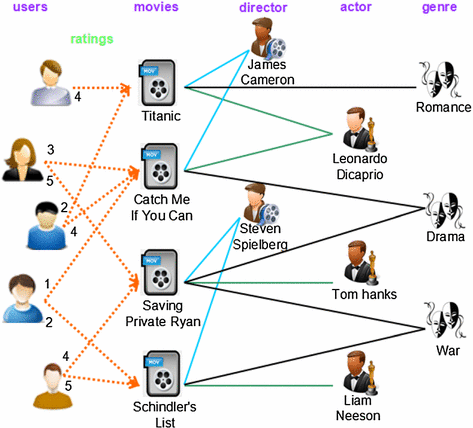
\includegraphics{graphics/user_matrix/usermatrix.JPG}
  \label{fig:usermatrix}
\end{figure}
The above image shows an illustration of a film recomendarion problem where there are multiple different items. these items being movies, director, actor and genre. these are also considered attributes of the film, through different methods such as a feedback system or through the user`s view history and search history. Which Film the user will be reccommended will depend greatly on the user-item rating matrix which is generally partly filles as it would be very time consuming for the user to submit feedback regareding each movie. Matrix Factorisation will attempt to reason out the ratings by transforming both users and items into the same favtor space.
Matrix models generally map both items and users into a joint latent dimensionality space f , such that the interactions between user and item are modelled as inner products. Each Item I is associated with a vector  f and each user u is associated with another vector f for each item I ,One of the main challenges is to compute the mapping of each user and item to the factor vectors. Once the mapping has been completed, the estimation process will take to give a compatibility rating for each item and user by performing the following equation
\begin{figure}
  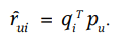
\includegraphics{graphics/user_matrix/usermatrix2.JPG}
  \label{fig:usermatrix2}
\end{figure}

\section{Learning Algorithms}
\index{Matrix Factorisation!Additional Input Sources|(}

The general idea behind ensembles is to merge each learner's hypothesis into one with the intention of obtaining better predictions. There are various ensemble methods, some of which use a single base learner to produce homogeneous learners while others use individual learners to produce heterogeneous learners. Generally, ensemble methods are applied to supervised learning algorithms. The methods described below are the most common used ensemble techniques in machine learning.



\index{Ensemble methods|)}